\setcounter{section}{0}
\setcounter{secnumdepth}{6}


% Typesets the font size, leading, and measure in the form of 10/12x26 pc.
\newcommand{\measure}[3]{#1/#2$\times$\unit[#3]{pc}}

% Macros for typesetting the documentation
\newcommand{\hlred}[1]{\textcolor{Maroon}{#1}}% prints in red
\newcommand{\hangleft}[1]{\makebox[0pt][r]{#1}}
\newcommand{\hairsp}{\hspace{1pt}}% hair space
\newcommand{\hquad}{\hskip0.5em\relax}% half quad space
\newcommand{\TODO}{\textcolor{red}{\bf TODO!}\xspace}
\newcommand{\na}{\quad--}% used in tables for N/A cells
\providecommand{\XeLaTeX}{X\lower.5ex\hbox{\kern-0.15em\reflectbox{E}}\kern-0.1em\LaTeX}
\newcommand{\tXeLaTeX}{\XeLaTeX\index{XeLaTeX@\protect\XeLaTeX}}
% \index{\texttt{\textbackslash xyz}@\hangleft{\texttt{\textbackslash}}\texttt{xyz}}
\newcommand{\tuftebs}{\symbol{'134}}% a backslash in tt type in OT1/T1
\newcommand{\doccmdnoindex}[2][]{\texttt{\tuftebs#2}}% command name -- adds backslash automatically (and doesn't add cmd to the index)
\newcommand{\doccmddef}[2][]{%
  \hlred{\texttt{\tuftebs#2}}\label{cmd:#2}%
  \ifthenelse{\isempty{#1}}%
    {% add the command to the index
      \index{#2 command@\protect\hangleft{\texttt{\tuftebs}}\texttt{#2}}% command name
    }%
    {% add the command and package to the index
      \index{#2 command@\protect\hangleft{\texttt{\tuftebs}}\texttt{#2} (\texttt{#1} package)}% command name
      \index{#1 package@\texttt{#1} package}\index{packages!#1@\texttt{#1}}% package name
    }%
}% command name -- adds backslash automatically
\newcommand{\doccmd}[2][]{%
  \texttt{\tuftebs#2}%
  \ifthenelse{\isempty{#1}}%
    {% add the command to the index
      \index{#2 command@\protect\hangleft{\texttt{\tuftebs}}\texttt{#2}}% command name
    }%
    {% add the command and package to the index
      \index{#2 command@\protect\hangleft{\texttt{\tuftebs}}\texttt{#2} (\texttt{#1} package)}% command name
      \index{#1 package@\texttt{#1} package}\index{packages!#1@\texttt{#1}}% package name
    }%
}% command name -- adds backslash automatically
\newcommand{\docopt}[1]{\ensuremath{\langle}\textrm{\textit{#1}}\ensuremath{\rangle}}% optional command argument
\newcommand{\docarg}[1]{\textrm{\textit{#1}}}% (required) command argument
\newenvironment{docspec}{\begin{quotation}\ttfamily\parskip0pt\parindent0pt\ignorespaces}{\end{quotation}}% command specification environment
\newcommand{\docenv}[1]{\texttt{#1}\index{#1 environment@\texttt{#1} environment}\index{environments!#1@\texttt{#1}}}% environment name
\newcommand{\docenvdef}[1]{\hlred{\texttt{#1}}\label{env:#1}\index{#1 environment@\texttt{#1} environment}\index{environments!#1@\texttt{#1}}}% environment name
\newcommand{\docpkg}[1]{\texttt{#1}\index{#1 package@\texttt{#1} package}\index{packages!#1@\texttt{#1}}}% package name
\newcommand{\doccls}[1]{\texttt{#1}}% document class name
\newcommand{\docclsopt}[1]{\texttt{#1}\index{#1 class option@\texttt{#1} class option}\index{class options!#1@\texttt{#1}}}% document class option name
\newcommand{\docclsoptdef}[1]{\hlred{\texttt{#1}}\label{clsopt:#1}\index{#1 class option@\texttt{#1} class option}\index{class options!#1@\texttt{#1}}}% document class option name defined
\newcommand{\docmsg}[2]{\bigskip\begin{fullwidth}\noindent\ttfamily#1\end{fullwidth}\medskip\par\noindent#2}
\newcommand{\docfilehook}[2]{\texttt{#1}\index{file hooks!#2}\index{#1@\texttt{#1}}}
\newcommand{\doccounter}[1]{\texttt{#1}\index{#1 counter@\texttt{#1} counter}}


\newcommand{\TL}{Tufte-\LaTeX\xspace}

% Prints the month name (e.g., January) and the year (e.g., 2008)
\newcommand{\monthyear}{%
  \ifcase\month\or January\or February\or March\or April\or May\or June\or
  July\or August\or September\or October\or November\or
  December\fi\space\number\year
}


% Prints an epigraph and speaker in sans serif, all-caps type.
\newcommand{\openepigraph}[2]{%
  %\sffamily\fontsize{14}{16}\selectfont
  \begin{fullwidth}
  \sffamily\large
  \begin{doublespace}
  \noindent\allcaps{#1}\\% epigraph
  \noindent\allcaps{#2}% author
  \end{doublespace}
  \end{fullwidth}
}

% Inserts a blank page
\newcommand{\blankpage}{\newpage\hbox{}\thispagestyle{empty}\newpage}

%%
% Prints argument within hanging parentheses (i.e., parentheses that take
% up no horizontal space).  Useful in tabular environments.
\newcommand{\hangp}[1]{\makebox[0pt][r]{(}#1\makebox[0pt][l]{)}}

%%
% Prints an asterisk that takes up no horizontal space.
% Useful in tabular environments.
\newcommand{\hangstar}{\makebox[0pt][l]{*}}

% commands not part of the style
\newcommand{\mypersec}{\si{\meter\per\second}}
\newcommand{\mympersecsq}{\si{\meter\per\second\squared}}
\newcommand{\mydegpersec}{\si{\degree\per\second}}
\newcommand{\mykm}{\si{\kilo\metre}}
\newcommand{\mym}{\si{\metre}}
\newcommand{\mymm}{\si{\milli\metre}}
\newcommand{\myum}{\si{\micro\metre}}
\newcommand{\myms}{\si{\milli\second}}
\newcommand{\myus}{\si{\micro\second}}
\newcommand{\myuw}{\si{\micro\watt}}
\newcommand{\myua}{\si{\micro\ampere}}
\newcommand{\myusr}{\si{\micro\steradian}}
\newcommand{\mydegree}{\si{\degree}}
\newcommand{\mymthreedb}{$-$3~dB}
\newcommand{\Unl}[1]{\ensuremath{\underline{#1}}}

\definecolor{LightGrey}{rgb}{0.96,0.96,0.96}
\definecolor{LightGrey}{rgb}{0.95,0.95,0.95}
\definecolor{light-gray}{gray}{0.95}
\definecolor{half-gray}{gray}{0.75}
\definecolor{LightRed}{rgb}{1.0,0.9,0.9}

\newcommand{\colheightrule}{\rule[-2mm]{0mm}{6.5mm}}
\newcommand{\marginnotecjw}[1]{ \marginpar{{\scriptsize #1}}}
\newcommand{\CJWpar}[2]{\parbox{#1}{\rule{0cm}{4mm}#2\rule[-2mm]{0cm}{4mm}}}
\newcommand{\HiLite}[1]{\fcolorbox{red}{red}{#1}}
\newcommand{\res}{\marginpar{$\ast$}}
\newcommand{\spec}[1]{\fcolorbox{half-gray}{light-gray}{#1}}

\newcommand{\TBC}[1]{%
    \par
    \noindent
    \begin{minipage}{1.0\linewidth}
      \begin{tcolorbox}[colback=purple!5, colframe=purple!95!black, coltext=black,
        coltitle=white, fonttitle=\bfseries, title={To be completed},%
        left=0mm, right=0mm, top=0mm, bottom=0mm,%
        before=\vspace{2pt}, after=\vspace{2pt}]
        % \setlength{\parskip}{0.5em} \vspace{-0.5em}
        %\setlength{\parindent}{1em} \noindent
        #1
        %\setlength{\parindent}{0em} \noindent
      \end{tcolorbox}
    \end{minipage}
}

\newcommand*\diff{\mathop{}\!\mathrm{d}}
\newcommand*\Diff[1]{\mathop{}\!\mathrm{d^#1}}
\newcommand*\euler{\mathop{}\!\mathrm{e}}
\newcommand*\imag{\mathop{}\!\mathrm{j}}

\newcommand{\mth}[1]{$#1$\textsuperscript{th}\ }

% set up the listings environment
%\begin{lstlisting}[hkey=value list]
%code here
%\end{lstlisting}
%\lstinline[hkey=value list]<character>source code<same character>
%\lstinputlisting[lastline=4]{listings.sty}

%\lstdefinelanguage{none}{identifierstyle=}

% set up listings package details
\lstloadlanguages{TeX,C++,XML,Python}


%\lstset{ %
\lstdefinestyle{ossimstyle}{
language=,                % choose the language of the code
upquote=true, % gives the upquote instead of the curly quote
basicstyle=\ttfamily\footnotesize,       % the size of the fonts that are used for the code
                  % alternative ((basicstyle=\ttfamily\fontsize{7}{10}\selectfont]))
numbers=none,                   % where to put the line-numbers (normally left)
numberstyle=\tiny,
%stepnumber=2,
numbersep=5pt,
showspaces=false,               % show spaces adding particular underscores
showstringspaces=false,         % underline spaces within strings
showtabs=false,                 % show tabs within strings adding particular underscores
breaklines=true,        % sets automatic line breaking
breakatwhitespace=false,    % sets if automatic breaks should only happen at whitespace
extendedchars=true,
keywordstyle=\color{red},
prebreak=\raisebox{0ex}[0ex][0ex]{$\dlsh$}, % add linebreak symbol
captionpos=b,                   % sets the caption-position to bottom
frame=none,                   % 'lines' or 'none' adds a frame around the code
%backgroundcolor=\color{LightGrey},
tabsize=2,              % sets default tabsize to 2 spaces
%escapeinside={\%}{)},          % if you want to add a comment within your code
%escapeinside={\%*}{*)},          % if you want to add LaTeX within your code
%backgroundcolor=\color{LightGrey},  % choose the background color,  add \usepackage{color}
framesep=1pt,
xleftmargin=0pt,
xrightmargin=0pt,
captionpos=t,                    % sets the caption-position to top
%deletekeywords={...},            % if you want to delete keywords from the given language
numberbychapter=false,
}

\DeclareCaptionFont{white}{\color{white}}
\DeclareCaptionFormat{listing}{\colorbox[cmyk]{0.43, 0.35, 0.35,0.01}{\parbox{\textwidth}{\hspace{15pt}#1#2#3}}}
\captionsetup[lstlisting]{format=listing,labelfont=white,textfont=white, singlelinecheck=false, margin=0pt, font={bf,footnotesize}}

% make inline listing larger than display
%https://latex.org/forum/viewtopic.php?t=2072
\makeatletter
\lst@AddToHook{TextStyle}{\let\lst@basicstyle\ttfamily\footnotesize\fontfamily{pcr}\selectfont}
\makeatother

\lstset{style=ossimstyle}


\lstdefinestyle{pythonstyle}{
  backgroundcolor=\color{LightGrey},  % choose the background colour,  add \usepackage{color}
  language=Python,
}

\lstdefinestyle{cppstyle}{
  backgroundcolor=\color{LightGrey},  % choose the background colour,  add \usepackage{color}
  language=C++,
}

\lstdefinestyle{xmlstyle}{
  backgroundcolor=\color{LightGrey},  % choose the background colour,  add \usepackage{color}
  language=XML,
}

\lstdefinestyle{nonestyle}{
  backgroundcolor=\color{LightGrey},  % choose the background colour,  add \usepackage{color}
}

\renewcommand{\arraystretch}{1.5}

\newcommand{\myhline}{\ \hrulefill \ }

%\minipsize{90mm}{some text}
\newcommand{\minipsize}[2]{\begin{minipage}[t]{#1}\begin{flushleft}#2\end{flushleft}\end{minipage}}


%%%%%%%%%%%%%%%%%%%%%%%%%%%%%%%%%%%%%%%%%%%%%%%%%%%%%%%%%%%%%
%\usepackage{etoolbox}
%\makeatletter
%\patchcmd{\thebibliography}{%
%  \chapter{\bibname}\@mkboth{\MakeUppercase\bibname}{\MakeUppercase\bibname}}{%
%  \chapter{References}}{}{}
%\makeatother

%\bibliographystyle{plain}
%\bibliographystyle{acm}
\bibliographystyle{bib/dpsscjw}

\newcommand{\tabrule}{\rule[-2mm]{0mm}{6mm}}

%% Symbols used in missile dynamics
%% See ../Missile Airframe-Guidance Models/c03_01.tex for definitions
\newcommand{\fax}{\ensuremath{f_\mathrm{ax}}}
\newcommand{\fay}{\ensuremath{f_\mathrm{ay}}}
\newcommand{\faz}{\ensuremath{f_\mathrm{az}}}
\newcommand{\fth}{\ensuremath{f_\mathrm{th}}}
\newcommand{\ribi}{\ensuremath{r_{ib}^i}}
\newcommand{\vibi}{\ensuremath{v_{ib}^i}}
\newcommand{\cib}{\ensuremath{C_i^b}}
\newcommand{\wibb}{\ensuremath{\omega_{ib}^b}}
\newcommand{\Wibb}{\ensuremath{\Omega_{ib}^b}}
\newcommand{\qdyn}{\ensuremath{q_\mathrm{dyn}}}
\newcommand{\sref}{\ensuremath{S_\mathrm{ref}}}
\newcommand{\vsound}{\ensuremath{v_\mathrm{s}}}
\newcommand{\nbt}{\ensuremath{\hat{t}}}
\newcommand{\tburn}{\ensuremath{t_\mathrm{burn}}}
\newcommand{\tign}{\ensuremath{t_\mathrm{ign}}}
\newcommand{\alphamax}{\ensuremath{\alpha_\mathrm{max}}}
\newcommand{\cazero}{\ensuremath{C_{A_0}}}
\newcommand{\cabase}{\ensuremath{C_{A_\mathrm{base}}}}
\newcommand{\cainc}{\ensuremath{C_{A_i}}}
\newcommand{\caincfull}{\ensuremath{C_{A_{if}}}}
\newcommand{\caincempty}{\ensuremath{C_{A_{ie}}}}
\newcommand{\cn}{\ensuremath{C_N}}
\newcommand{\cnfull}{\ensuremath{C_{N_f}}}
\newcommand{\cnempty}{\ensuremath{C_{N_e}}}
\newcommand{\xref}{\ensuremath{X_\mathrm{ref}}}
\newcommand{\czalpha}{\ensuremath{{C_{Z_\alpha}}}}
\newcommand{\chk}{$\times$}


\newcommand{\formatpart}[1]{%
\begin{fullwidth}
    \centering%
    \partname~\thepart%
    \newline%
    \ \newline%
    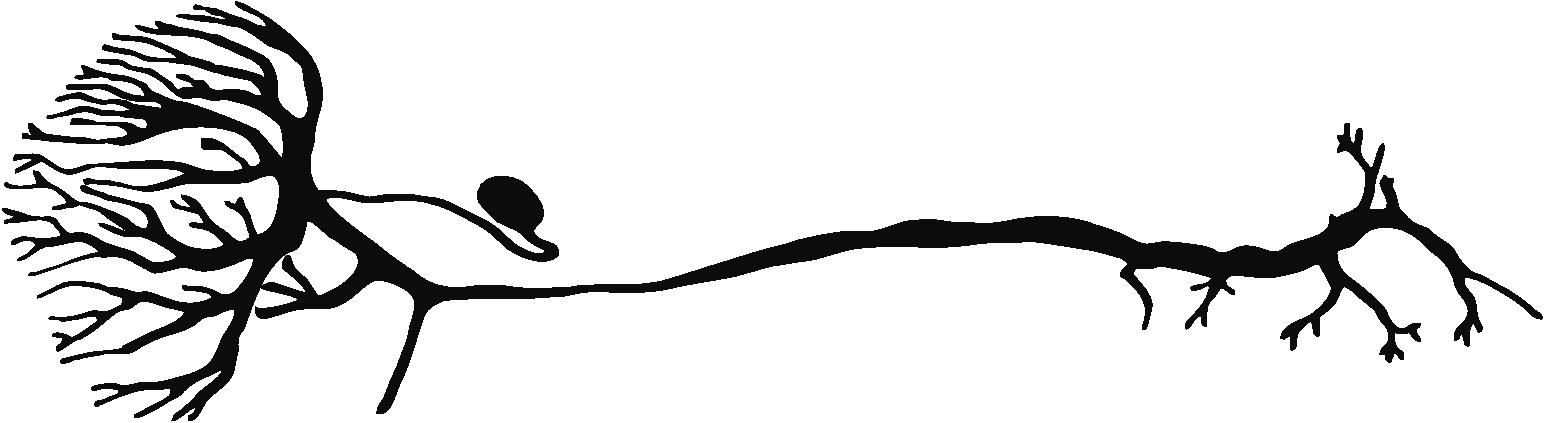
\includegraphics[width=.7\textwidth,]{pic/neuronstylised}%
    \ \newline%
    \ \newline%
    #1%
\end{fullwidth}
    }


%the following is required for carriage return symbol
%ftp://ftp.botik.ru/rented/znamensk/CTAN/fonts/mathabx/texinputs/mathabx.dcl
%https://secure.kitserve.org.uk/content/mathabx-font-symbol-redefinition-clash-latex
\DeclareFontFamily{U}{mathb}{\hyphenchar\font45}
\DeclareFontShape{U}{mathb}{m}{n}{
      <5> <6> <7> <8> <9> <10> gen * mathb
      <10.95> mathb10 <12> <14.4> <17.28> <20.74> <24.88> mathb12
      }{}
\DeclareSymbolFont{mathb}{U}{mathb}{m}{n}
\DeclareMathSymbol{\dlsh}{3}{mathb}{"EA}


% redefine parindent and parskip for Tufte class
%https://tex.stackexchange.com/questions/77999/remove-indent-of-paragraph-and-add-line-skip-with-tufte-latex
\makeatletter
% Paragraph indentation and separation for normal text
\renewcommand{\@tufte@reset@par}{%
  \setlength{\RaggedRightParindent}{0pt}%
  \setlength{\JustifyingParindent}{0pt}%
  \setlength{\parindent}{0pt}%
  \setlength{\parskip}{0.3\bigskipamount plus \smallskipamount minus \smallskipamount}%
}
\@tufte@reset@par

% Paragraph indentation and separation for marginal text
\renewcommand{\@tufte@margin@par}{%
  \setlength{\RaggedRightParindent}{0pt}%
  \setlength{\JustifyingParindent}{0pt}%
  \setlength{\parindent}{0pt}%
  \setlength{\parskip}{0.3\bigskipamount plus \smallskipamount minus \smallskipamount}%
}
\makeatother


